\section{Modelagem e Aplicação}
	Com a finalidade de validar a interface proposta neste trabalho, foi construído um ambiente virtual baseado nas características de um ambiente real (escritório). Estás características foram obtidas com o auxílio da planta baixa do ambiente proposto, ilustrada pela Figura~\ref{fg:planta_baixa}.

\begin{figure}[!ht]
	\centering
	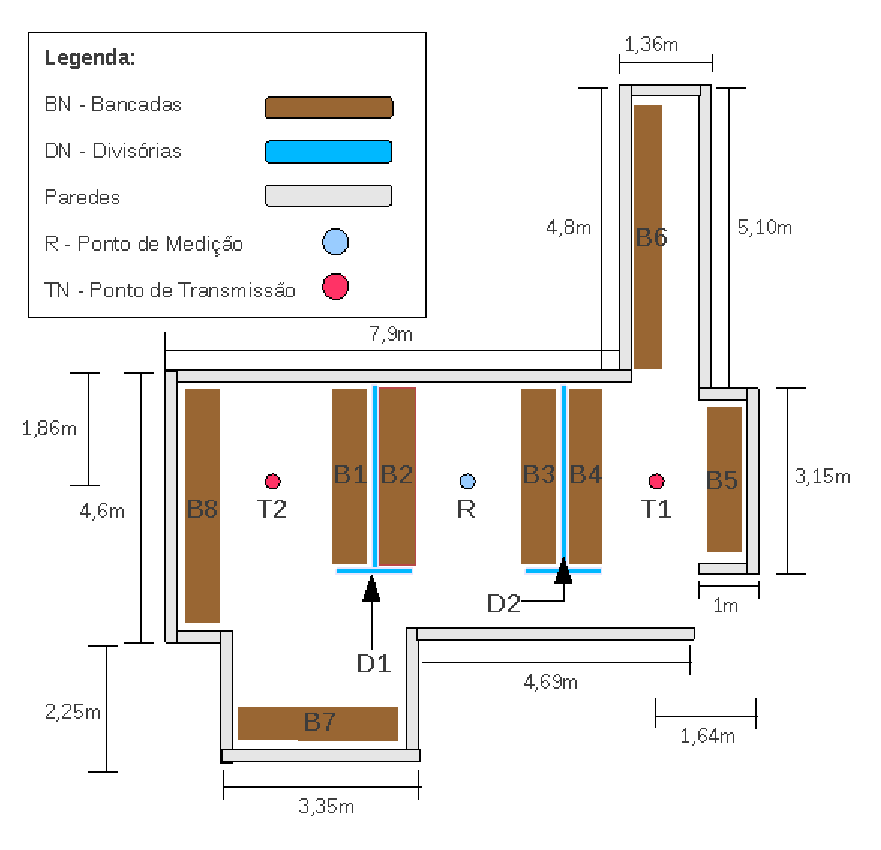
\includegraphics[scale = 1]{planta_baixa}
	\caption{Planta baixa do ambiente simulado e pontos de transmissão e recepção.}
	\label{fg:planta_baixa}
\end{figure}

	Neste ambiente, utilizando o modelo numérico aqui desenvolvido, foram feitos registro transitórios do campo elétrico transmitido por uma antena banda larga em pontos específicos do cenário (mantendo a porta fechada), o que possibilitou a obtenção da resposta à propagação do sinal desta antena.

	A maioria dos objetos presentes no ambiente real, no momento da realização das medições experimentais~\cite{fabricio}, foram modelados. As especificações destes objetos estão na Tabela~\ref{tb:objetos}.

\begin{table}
	\centering
	\caption{Objetos e suas dimensões.}
	\begin{tabular}{|l|l|l|l|}
	\hline
	\textbf{Objetos} & \textbf{Dimensão $X$} & \textbf{Dimensão} $Y$ & \textbf{Dimensão $Z$}\\ \hline
	Computadores (gabinetes) & 0,18m & 0,43m & 0,42m \\ \hline
	Monitores & 0,39m & 0,31m & 0,39m \\ \hline
	Divisórias 1 e 2 & 3,27m & 1,5m & 0,03m \\ \hline
	Paredes divisórias 1 e 2 & 0,03m & 1,5m & 1m \\ \hline
	Bancadas de 1-4 & 3,21m & 0,03m & 0,5m \\ \hline
	Bancada 5 & 2,94m & 0,03m & 0,5m \\ \hline
	Bancada 6 & 4,68m & 0,03m & 0,5m \\ \hline
	Bancada 7 & 0,5m & 0,03m & 3,18m \\ \hline
	Bancada 8 & 4,26m & 0,03m & 0,5m \\
	\hline
	\end{tabular}
	\label{tb:objetos}
\end{table}

	Alguns destes objetos estão dispostos em alturas diferentes em relação ao piso. As bancadas e o teto estão a uma altura de 0,75 metro e 2,73 metros, respectivamente. Os computadores e monitores foram colocados na célula imediatamente acima do nível das bancadas. Dessa forma, o plano relativo às bases dos computadores coincide com o plano das bancadas.

	As dimensões gerais desse cenário usadas na interface foram:
\begin{itemize}
\item \textit{$\Delta$}(Aresta da célula de Yee) utilizada foi de $0,03m$.
\item \textit{Região de Análise} com dimensões: $X$ = $15m$, $Y$ = $3m$ e $Z$ = $15m$.
\item \textit A lista das caraterísticas físicas com seus respectivos materiais é representada na Tabela~\ref{tab:materiais}~\cite{fabricio}.
\end{itemize}

\begin{table}
	\centering
	\caption{Tabela de materiais e parâmetros físicos.}
	\begin{tabular}{|l|l|l|l|l|}
	\hline
	Elementos dos Ambiente & Material & $\epsilon_r$ & $\sigma$ & $\mu_r$ \\ \hline
	Parede & Tijolo & $4$ & $0,0135$ & $1$\\ \hline
	Teto & Gesso & $2,8$ & 0,1533 & 1 \\ \hline
	Bancadas & Madeira & $1,8$ & $0,011$ & $1$\\ \hline
	Monitores e Gabinetes & Metal & $5$ & $1\times10^{11}$ & $1$\\ \hline
	Divisórias & Vidro & $5$ & $5\times10^{-4}$ & $1$ \\ \hline
	Piso & Concreto & $5$ & $1$ & $1$ \\
	\hline
	\end{tabular}	
	\label{tab:materiais}
\end{table}

	As características do solo (abaixo do piso) são as de um meio rochoso. Os parâmetros $\epsilon_r=50$ e $\mu_r=2{,}28$, para este tipo de solo, foram obtidas em~\cite{tanabe}.

	O resultado da modelagem (usando a interface) foi o conjunto das estruturas mostradas nas Figuras~\ref{fg:ambiente} e \ref{fg:amb_sags} . A disposição dos objetos no AV, foi realizada de forma a corresponder com o posicionamento real no momento das medições experimentais ~\cite{fabricio}. As Figuras~\ref{fg:corredor}, \ref{fg:bancada} e \ref{fg:outrav} mostram o ambiente modelado e seus objetos com mais detalhe.

\begin{figure}[!ht]
	\centering
	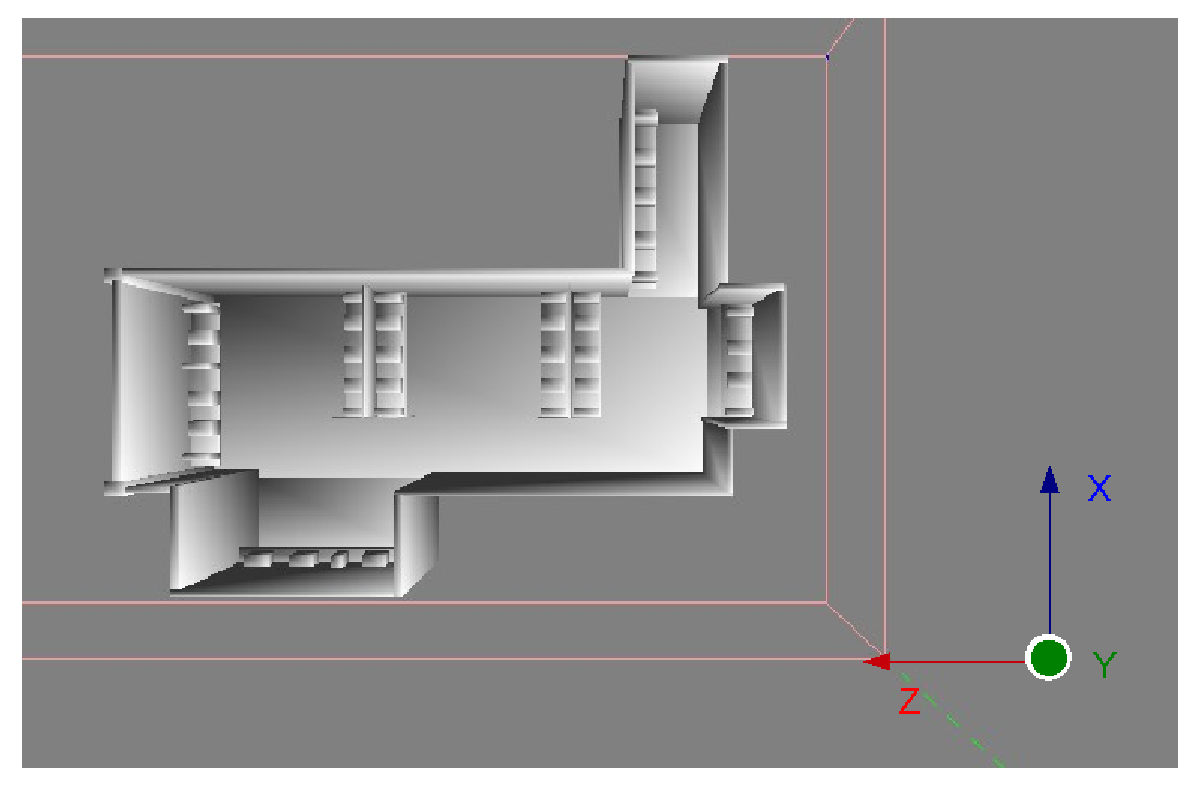
\includegraphics[scale = 0.4]{ambiente}
	\caption{Visão superior do ambiente modelado neste trabalho.}
	\label{fg:ambiente}
\end{figure}
\begin{figure}[!tp]
	\centering
	\includegraphics[scale = 0.4]{amb_sags}
	\caption{Visão em perspectiva do cenário no simulador LANE-SAGS.}
	\label{fg:amb_sags}
\end{figure}
\begin{figure}[!ht]
	\centering
	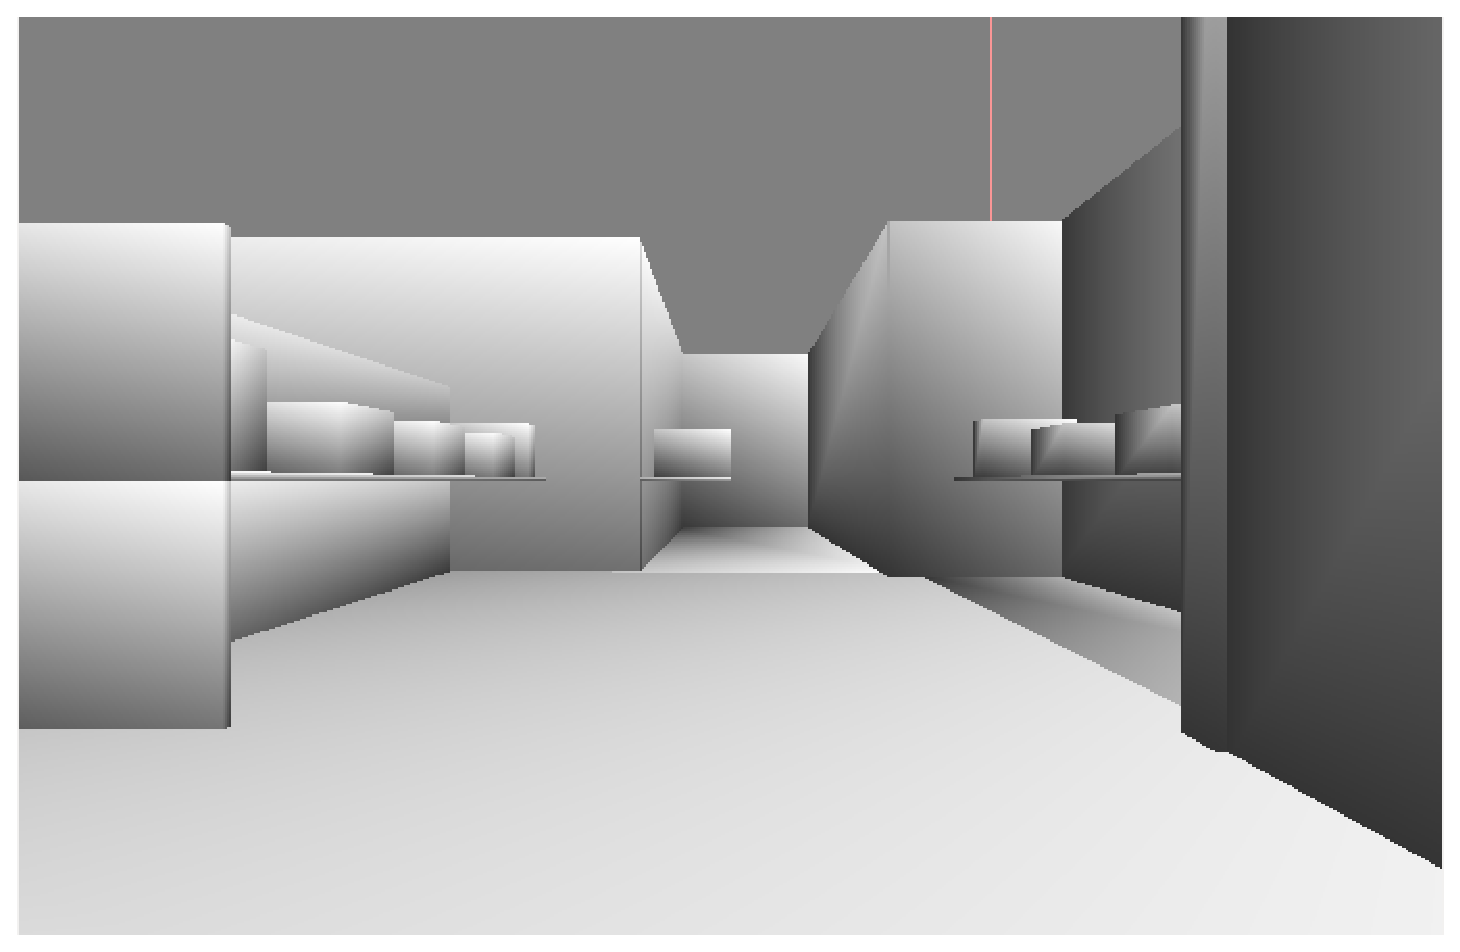
\includegraphics[scale = 0.4]{corredor}
	\caption{Visão interna do ambiente modelado (corredor 1).}
	\label{fg:corredor}
\end{figure}
\begin{figure}[!ht]
	\centering
	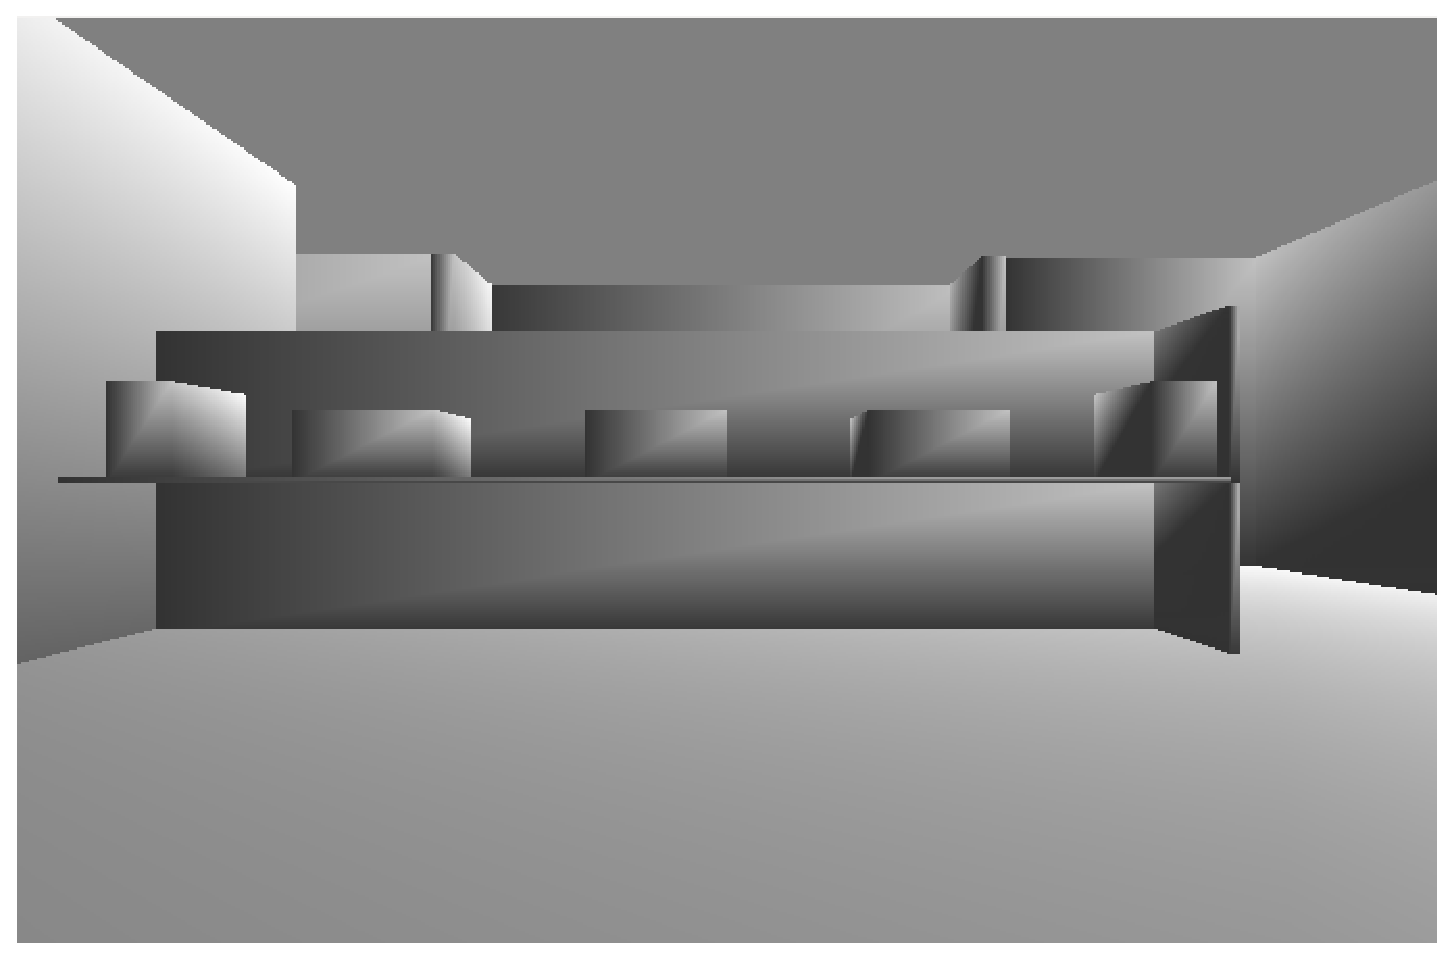
\includegraphics[scale = 0.4]{bancada}
	\caption{Visão interna do ambiente modelado (bancada).}
	\label{fg:bancada}
\end{figure}
\begin{figure}[!ht]
	\centering
	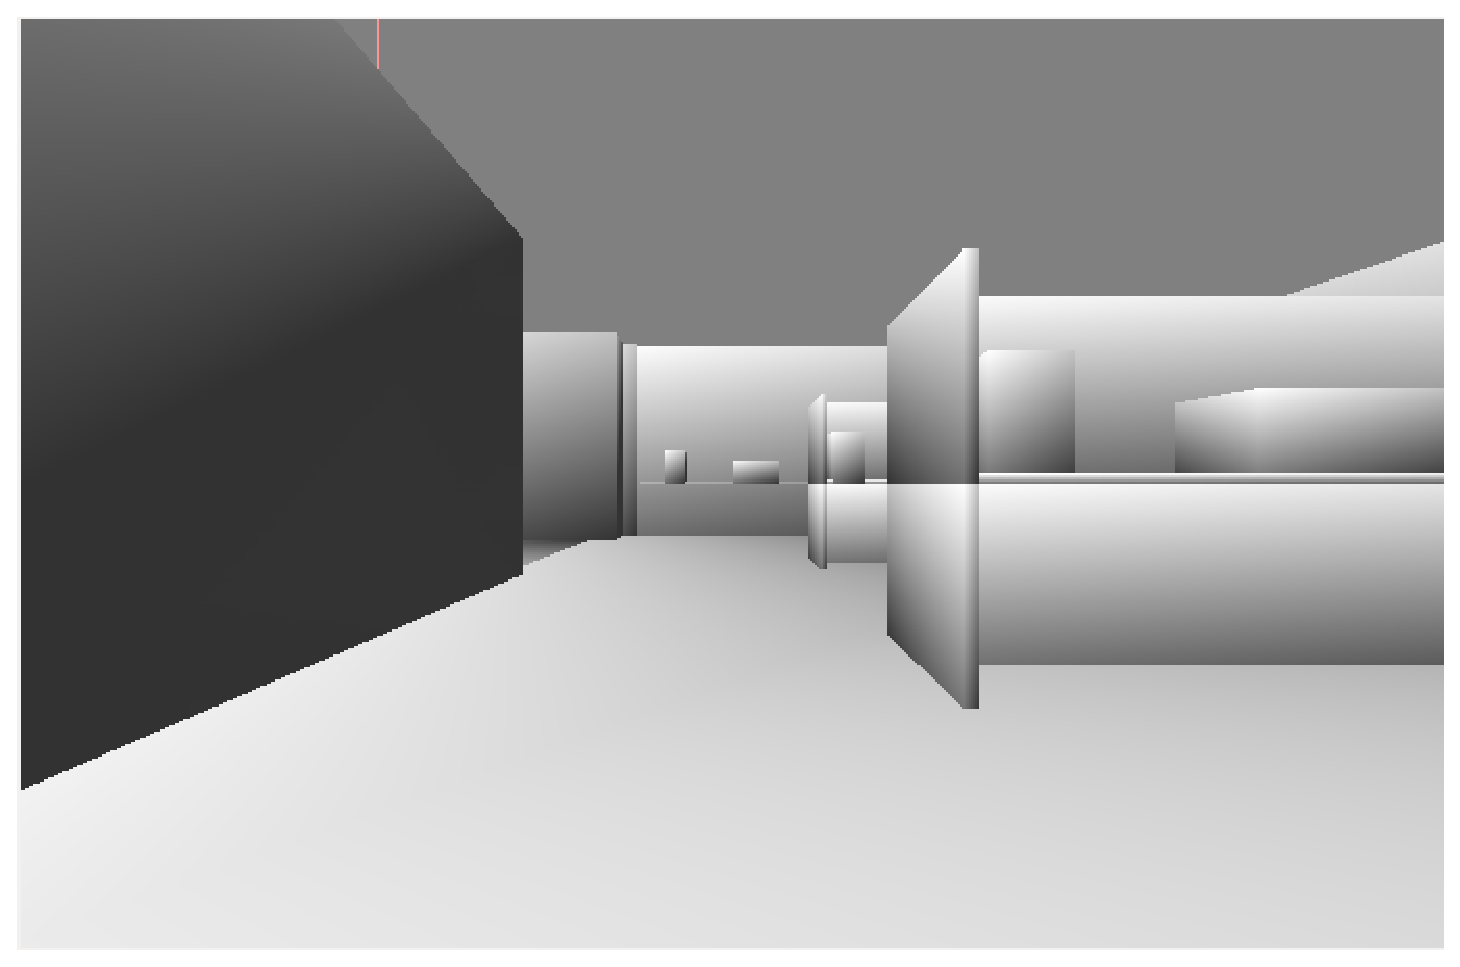
\includegraphics[scale = 0.4]{outrav}
	\caption{Visão interna do ambiente modelado (corredor 2).}
	\label{fg:outrav}
\end{figure}


\subsection{Criação e Introdução da Antena}

	Depois de o ambiente ter sido modelado na interface, surgiu a necessidade de introduzir a antena. Como a que foi usada no experimento era altamente complexa (antena discônica), foi necessário projetar um antena com geometria mais simples, mas que de forma semelhante à real. Após fazer uma análise, percebeu-se que antena usada durante as experimentações~\cite{fabricio} funcionava como dipolo. Desta forma, alguns teste foram realizados, de forma a obter um representação aceitável para a antena. Esta deveria ter um diagrama omnidirecional e perda de retorno abaixo de -10dB na faixa de frequência de interesse. 

	Para todos os modelos de antenas testados, foi utilizada uma sinal que varia no tempo de acordo com a função monociclo gaussiano (derivada do pulso gaussiano), tal como descrito matematicamente por (\ref{eq:trem}) e graficamente pela Figura~\ref{fg:tensao}. Utilizou-se a transformada de Fourier para verificar se a faixa de frequência, do sinal usado, esta na banda adequada (entre 700MHz-900MHz). O espectro do sinal monociclo gaussiano (\ref{eq:trem}) é ilustrado pela Figura~\ref{fg:f_fonte}.

\begin{equation}\label{eq:trem}
	f(t) = A_{p}\exp \left( - \left( \frac{t-3.0\ T}{T}  \right)^2 \right )  \left( \frac{t-3T}{T} \right)
\end{equation}
Onde:\\
$A_p = 1$ e $T$ =  $6.53846\times10^{-10}$
\begin{figure}[!ht]
	\begin{center}
		\subfigure[Gráfico da fonte no tempo.]{\label{fg:tensao}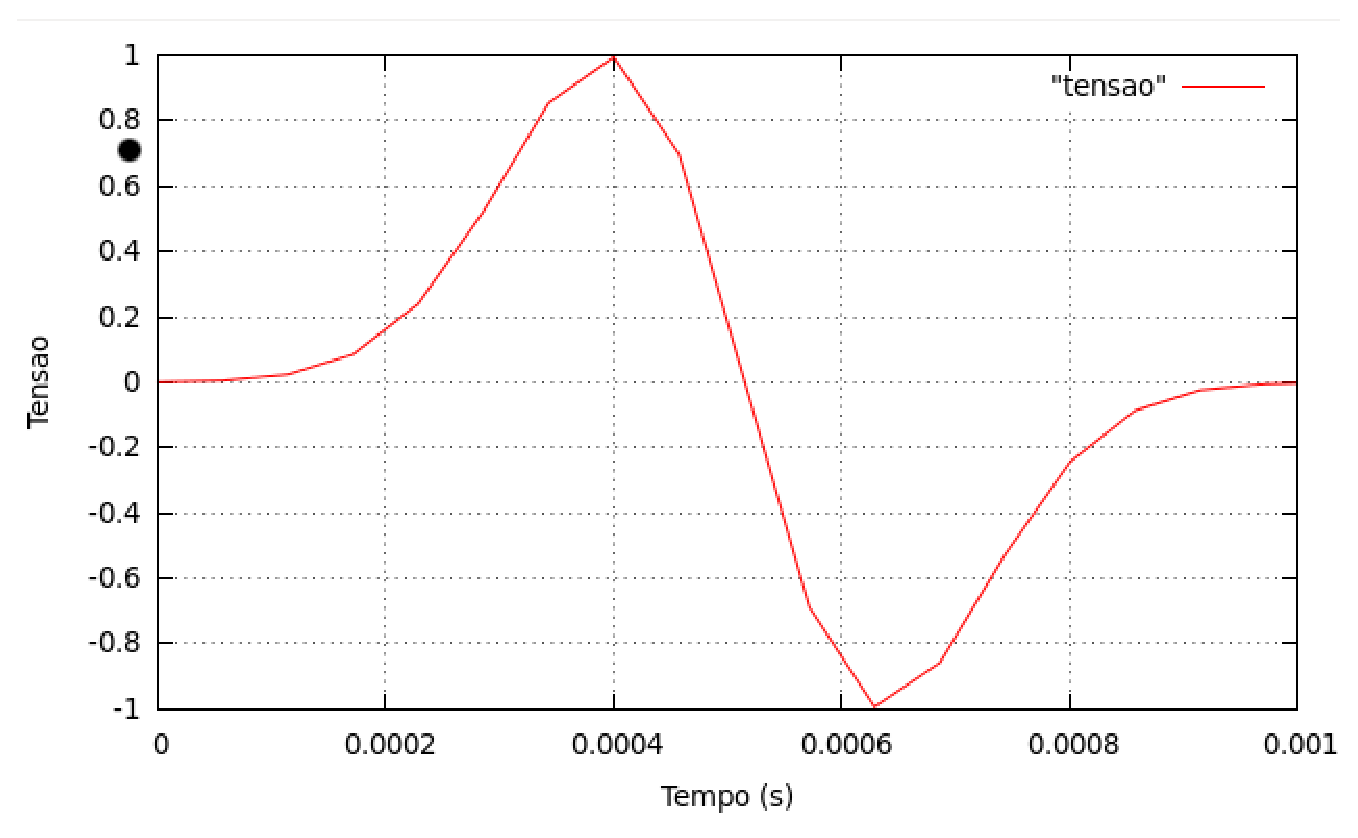
\includegraphics[scale=0.3]{tensao}}
\qquad
		\subfigure[Gráfico da transformada de Fourier da fonte.]{\label{fg:f_fonte}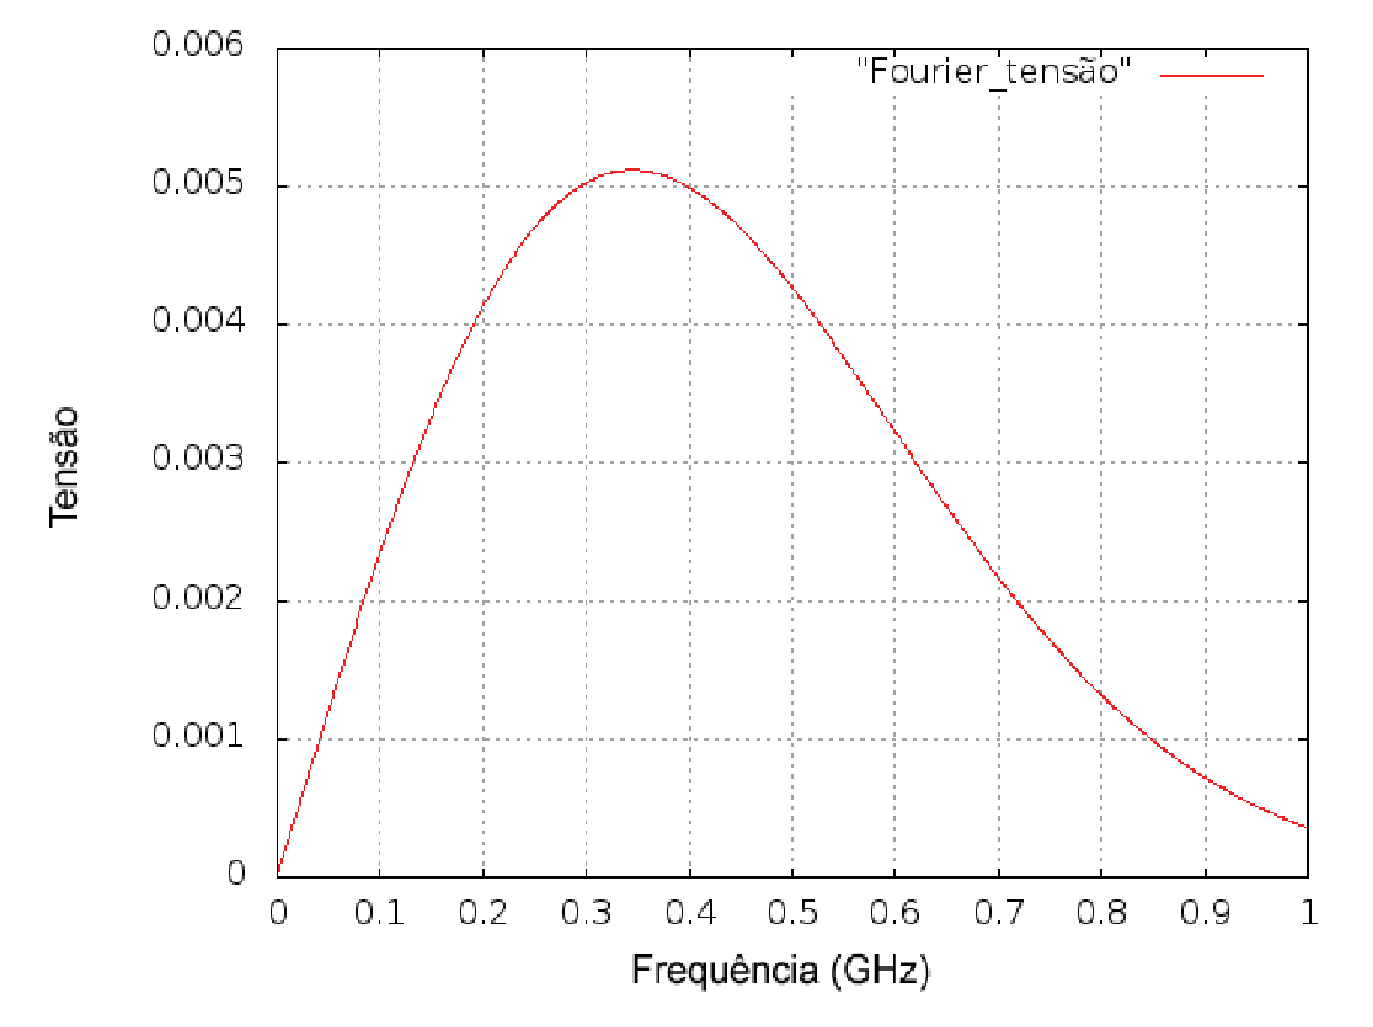
\includegraphics[scale=0.3]{f_fonte}}
	\end{center}
	\caption{Fonte de tensão usada para excitar as antenas modeladas.}
	\label{fg:fontes}
\end{figure}

	A primeira antena-teste montada ilustrada pela Figura~\ref{fg:antena_normal}, juntamente com sua representação no LANE-SAGS(Figura~\ref{fg:antena_normal_sags}). Esta antena dipolo é similar a usada em~\cite{josivaldo}. Os dois blocos têm as mesmas dimensões, assim como as duas hastes metálicas. Entre os terminais da antena (espaço entre as duas hastes), a tensão mostrada na Fig.~\ref{fg:tensao} foi estabelecida através da excitação do campo elétrico. Para fins de projeto, foi calculada a corrente transitória em uma das hastes (na célula vizinha à célula de excitação do campo elétrico) por meio do rotacional do campo magnético que circunda ao redor da haste.

\begin{figure}[!ht]
	\begin{center}
		\subfigure[Projeto inicial de antena.]{\label{fg:antena_normal}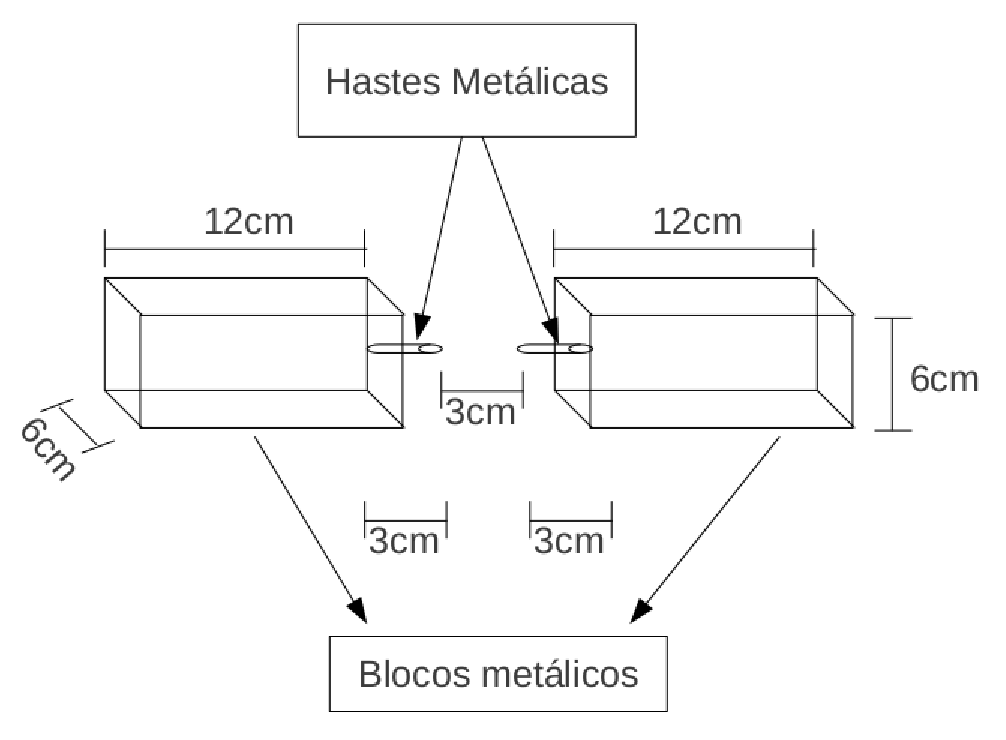
\includegraphics[scale=0.3]{antena_normal}}
\qquad
		\subfigure[Visualização do protótipo no simulador LANE-SAGS.]{\label{fg:antena_normal_sags}\includegraphics[scale=0.25]{antena_normal_sags}}
	\end{center}
	\caption{Antena dipolo tradicional.}
	\label{fg:antena_normal_m}
\end{figure}

	Com os dados transitório de tensão $V(t)$ e corrente $I(t)$, foi calculado o coeficiente de reflexão através da relação~\ref{eq:impedancia}. Em (~\ref{eq:impedancia}), $Z$ é a impedância da antena, dada por $Z$ = $F(V(t)/F(I(t)))$, onde $F$ é o operador da transformada de Fourier e $Z_S = 50\Omega$ é a impedância da carga. Por meio deste coeficiente $\Gamma$, pode-se calcular a perda de retorno, associada a essa antena(Equação~\ref{eq:pr}). Como pode-se observar na  Figura~\ref{fg:pr_01}, a antena está trabalhando abaixo de -10dB em uma faixa diferente da desejada (700MHz-900MHz). Portanto, suas dimensões e parâmetros necessitaram ser modificados.

\begin{figure}[!ht]
	\centering
	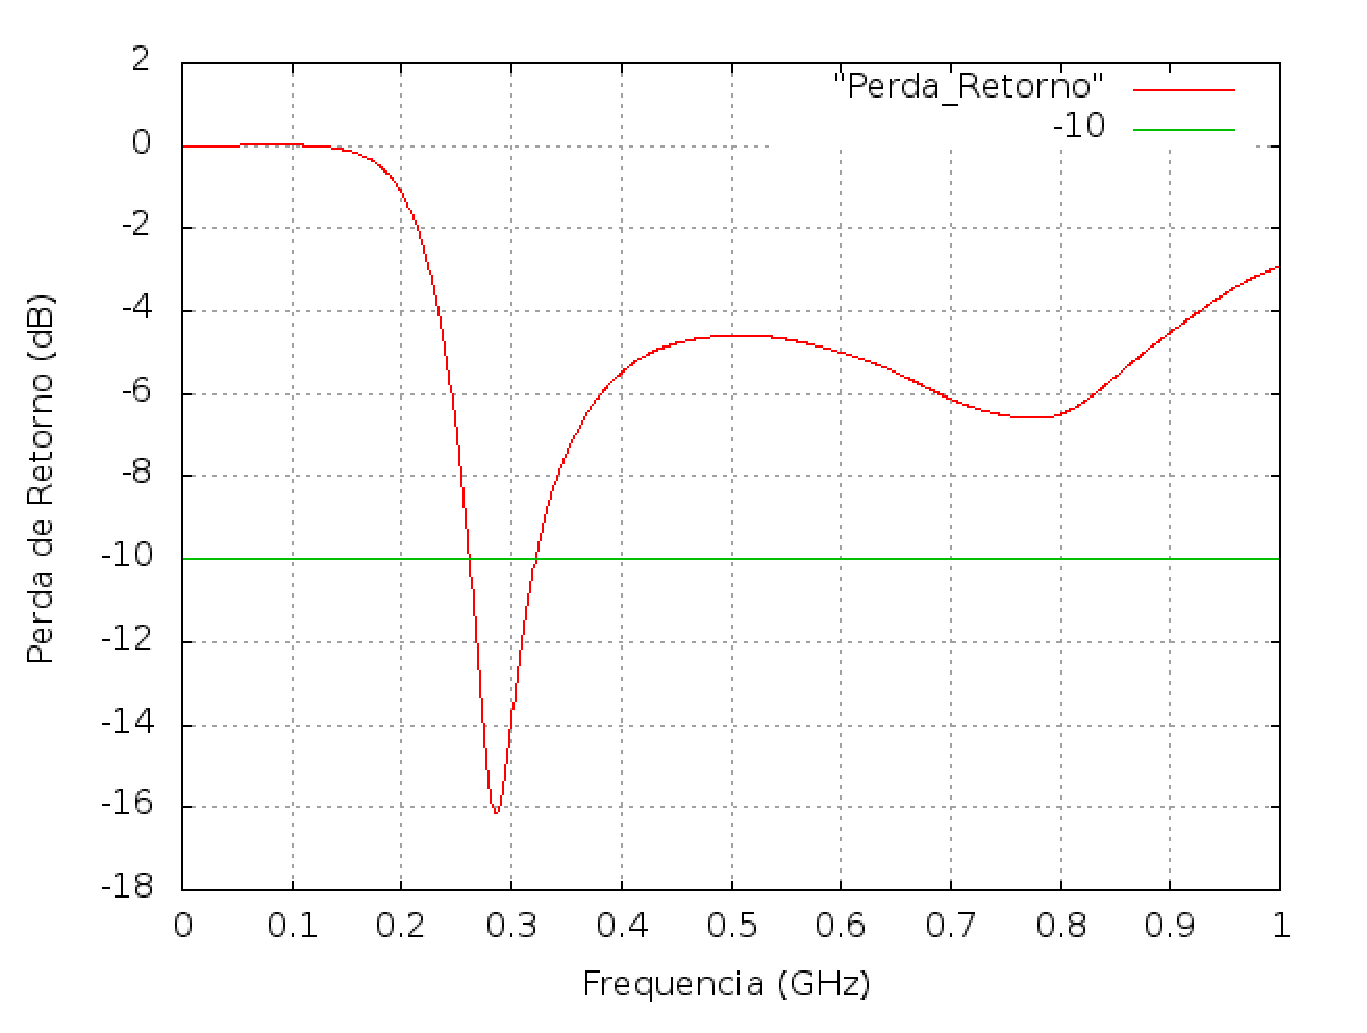
\includegraphics[scale = 0.5]{pr_01}
	\caption{Perda de retorno da antena dipolo tradicional(primeira antena modelada).}
	\label{fg:pr_01}
\end{figure}

\begin{equation}\label{eq:impedancia}
	\Gamma = \frac{Z - Z_{S}}{Z + Z_{S}}
\end{equation}

\begin{equation}\label{eq:pr}
	RL(dB) = -20log_{10} |\Gamma|
\end{equation}

	Após alguns testes, verificou-se que a diminuição na dimensão dessa antena afetava de forma positiva o resultado da perda de retorno. Porém, havia um problema ligado ao comprimento das arestas de célula de Yee ($\Delta$), que diminuiria de forma proporcional à redução das dimensões da antena, inviabilizando as simulações devido ao alto custo computacional relativo ao método FDTD. Para solucionar este impasse, optou-se pelo uso de um capacitor ($3,7\times10^{-5}$ farad) acoplado a um dos blocos metálicos, afim de sintonizar a antena com a banda de interesse (casamento de impedâncias). Este arranjo possibilitou o uso da antena sem alterar suas dimensões (tamanho) e, principalmente, sem modificar o parâmetro $\Delta$. Sabe-se que o aumento do comprimento da antena deixa-a indutiva e que a antena dipolo é omnidirecional~\cite{balanes}.

	A configuração da antena adaptada está ilustrada na Figura~\ref{fg:antena_final}. A Figura~\ref{fg:antena_final_sags} mostra o modelo no LANE-SAGS. Todos os cálculos tiveram que ser refeitos para nova antena, obtendo-se a perda de retorno desejada. A Figura~\ref{fg:pr_2} mostrada os resultados para a antena adaptada (em vermelho) e para a antena original (em verde). 

\begin{figure}[!ht]
	\centering
	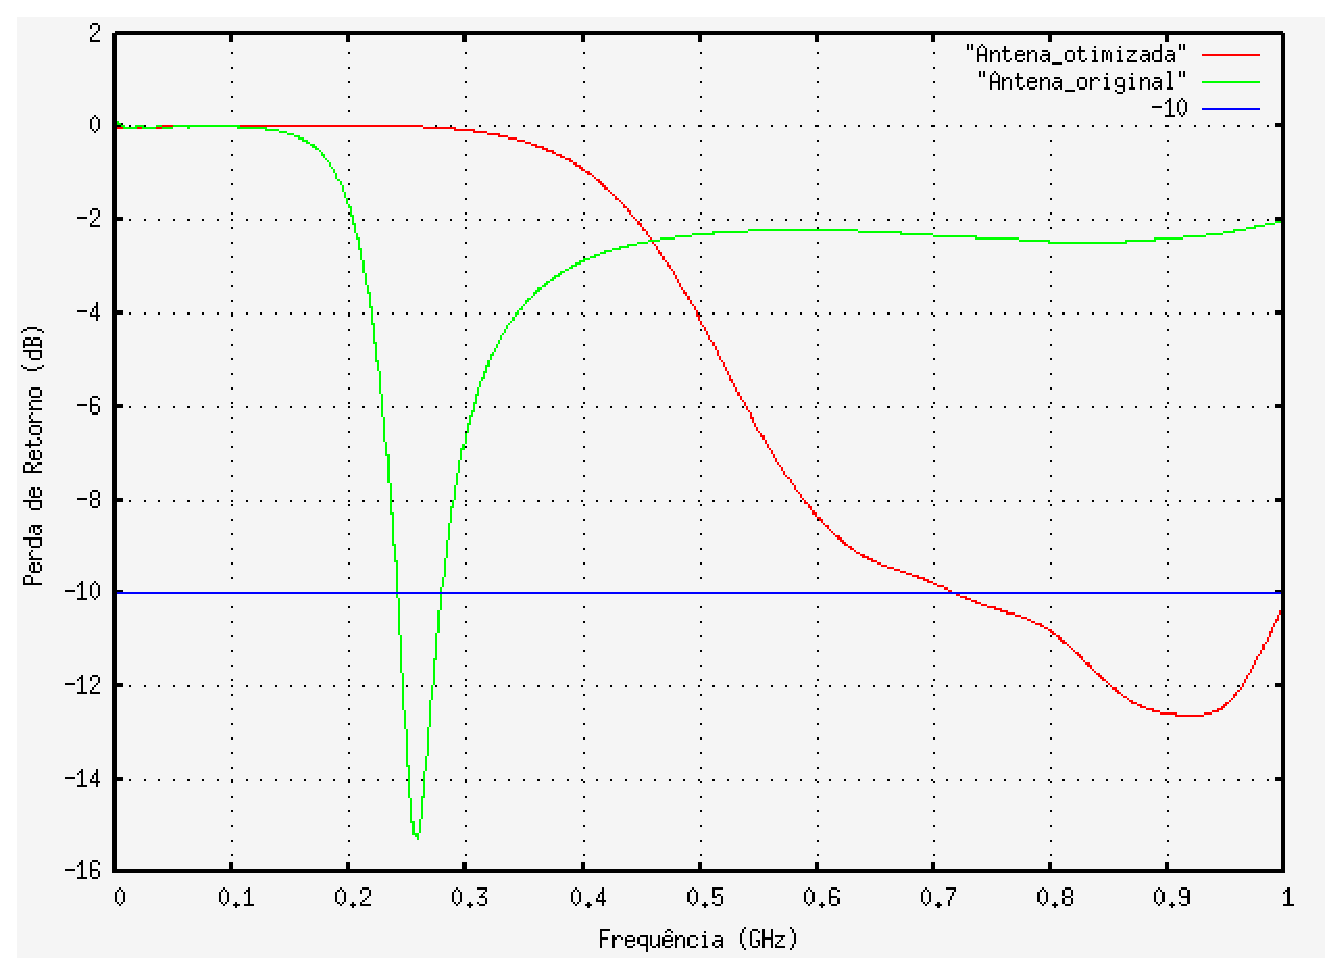
\includegraphics[scale = 0.5]{pr_2}
	\caption{Comparação entre as perdas de retorno da antena otimizada(adaptada) e normal(original).}
	\label{fg:pr_2}
\end{figure}

\begin{figure}[!ht]
	\begin{center}
		\subfigure[Diagrama da antena dipolo adaptada.]{\label{fg:antena_final}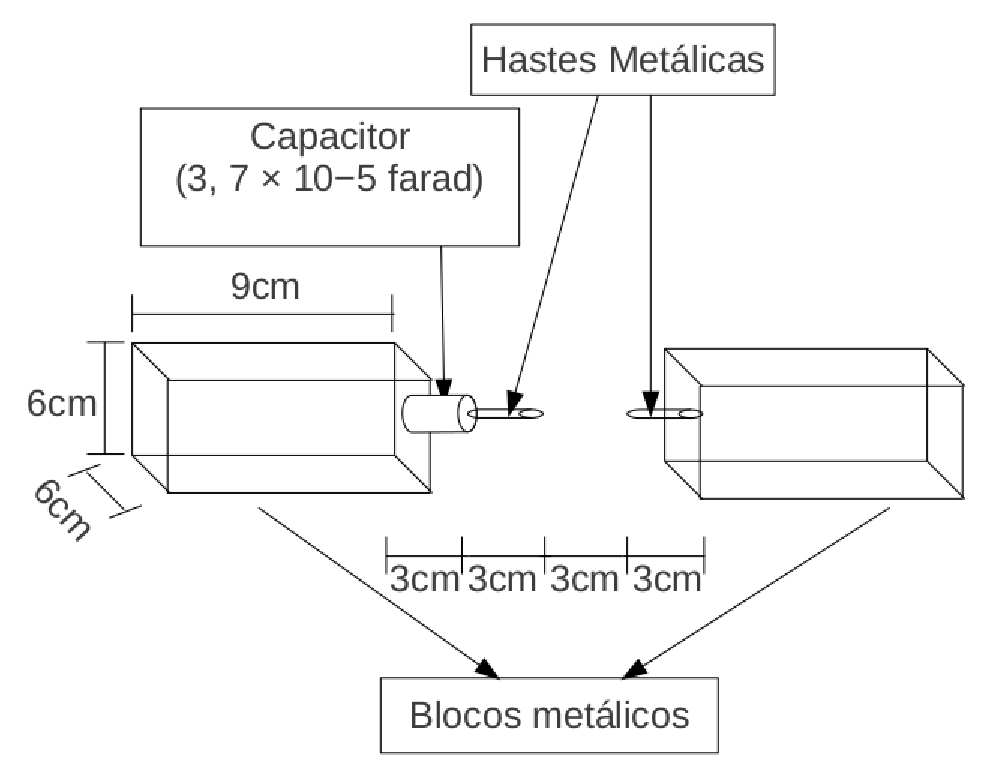
\includegraphics[scale=0.3]{antena_final}}
\qquad
		\subfigure[Visualização da antena adaptada no simulador LANE-SAGS.]{\label{fg:antena_final_sags}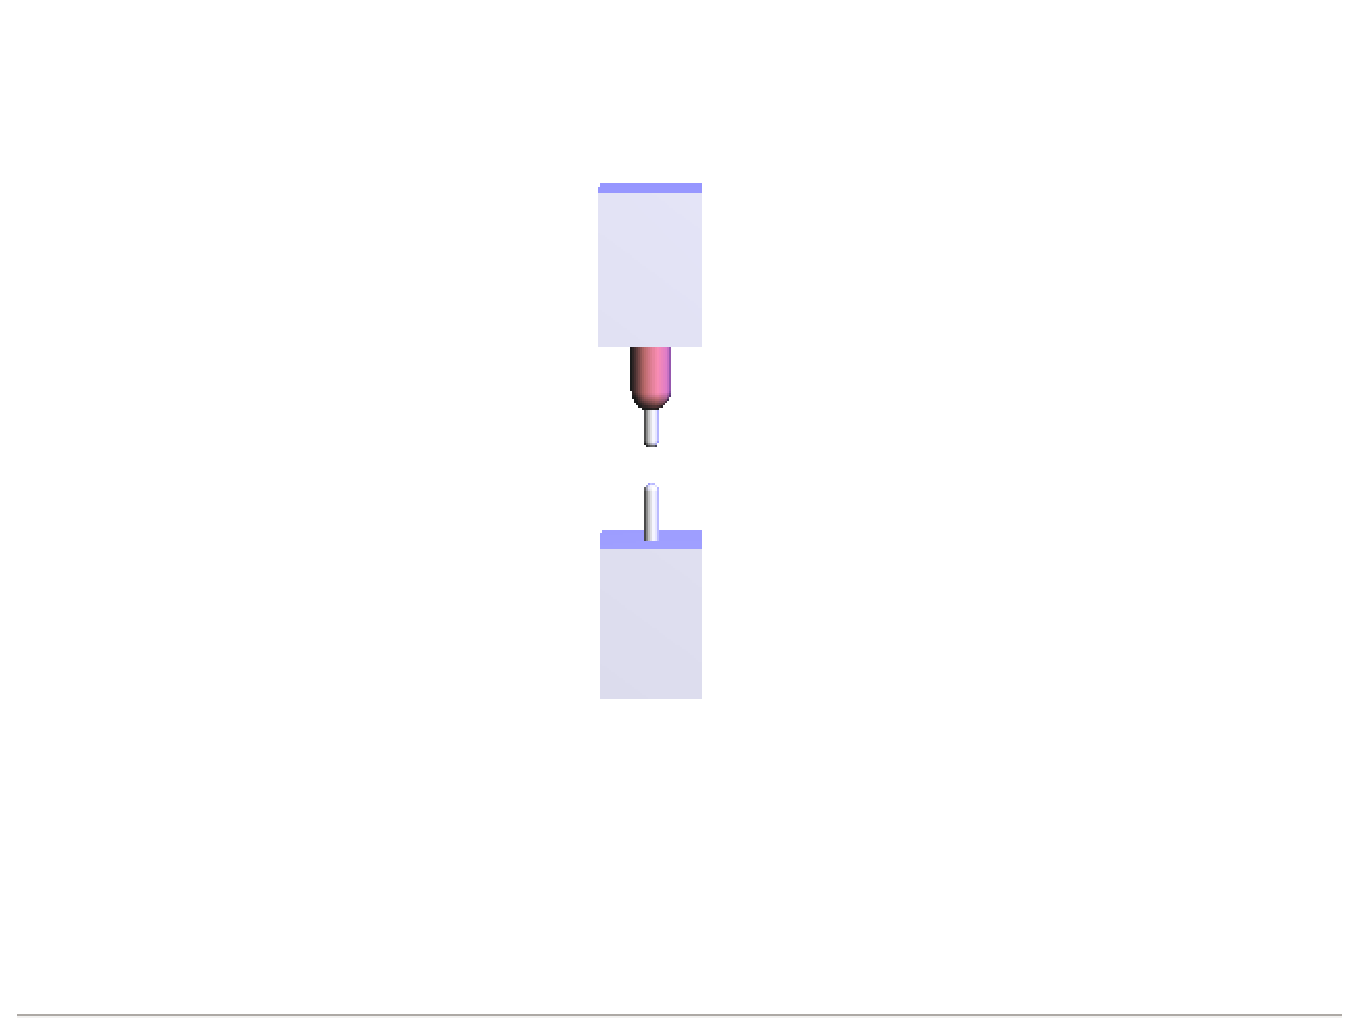
\includegraphics[scale=0.25]{antena_final_sags}}
	\end{center}
	\caption{Antena dipolo adaptada.}
	\label{fg:antena_aptada}
\end{figure}

\subsection{Resultados}
\subsubsection{Caso 01}
	O caso 01 refere-se à introdução da antena modelada na posição T1 da Figura~\ref{fg:planta_baixa}. Ela foi posicionada a uma altura de 1,5m do piso e polarizada em $z$. Com isso, foi feita a simulação da propagação do pulso monociclo Gaussiano a partir da antena projetada. Obteve-se, além da tensão calculada no ponto R(mesma altura do ponto T1) do cenário modelado, a tensão entre nos terminais da antena transmissora. Esse sinais estão mostrados nas Figuras~\ref{fg:t_out} e \ref{fg:t_in}, respectivamente.

\begin{figure}[!ht]
	\begin{center}
		\subfigure[Gráfico da tensão no Ponto R.]{\label{fg:t_out}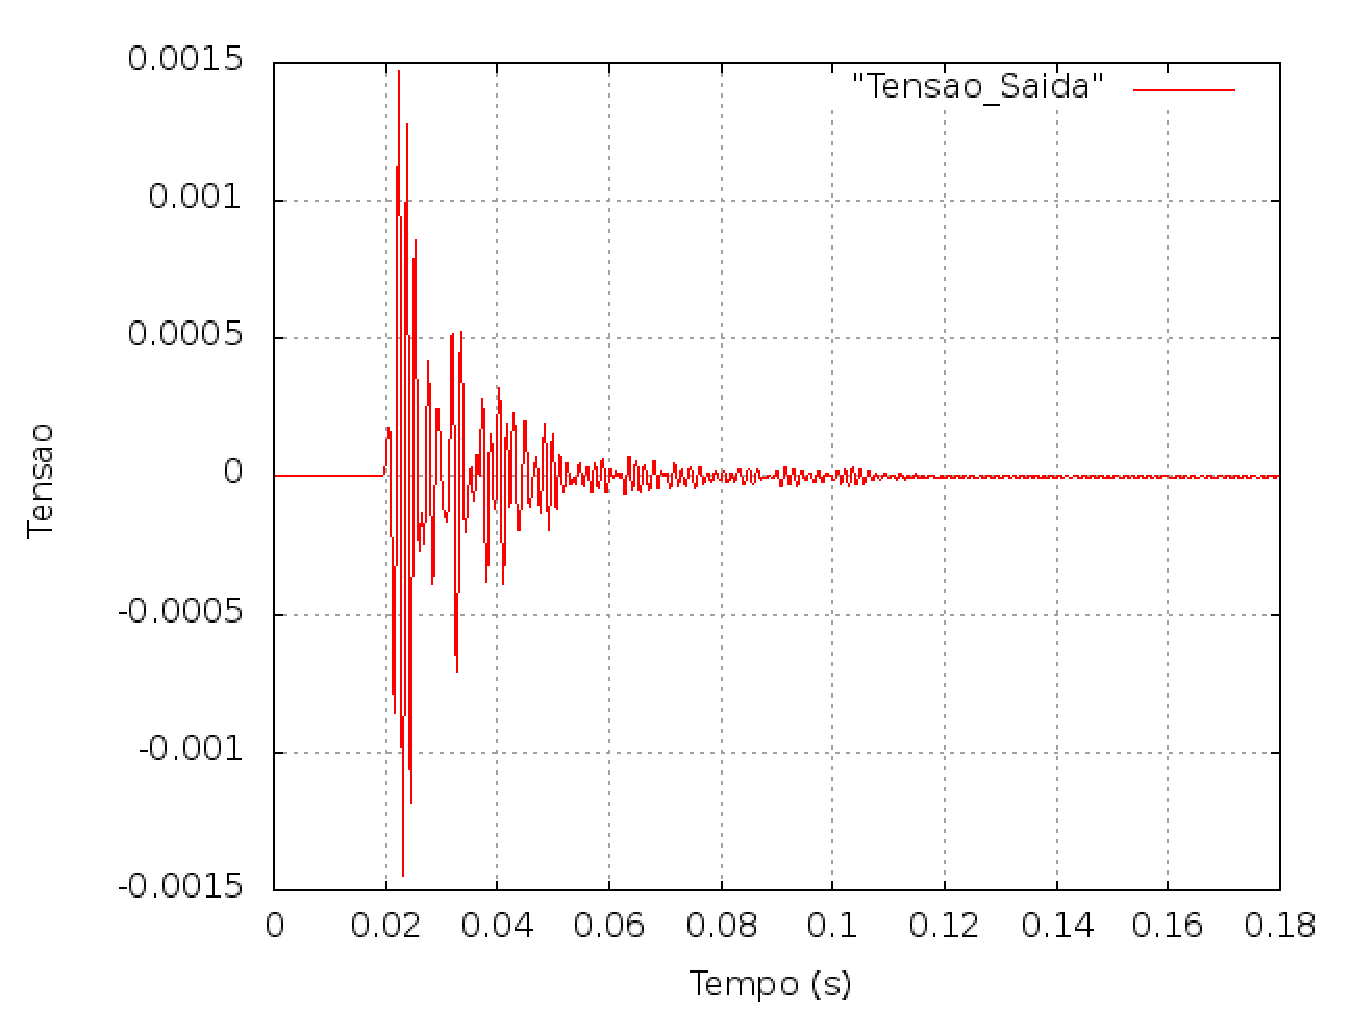
\includegraphics[scale=0.25]{t_out}}
\qquad
		\subfigure[Gráfico da tensão no Ponto $T1$(entre as hastes da antena).]{\label{fg:t_in}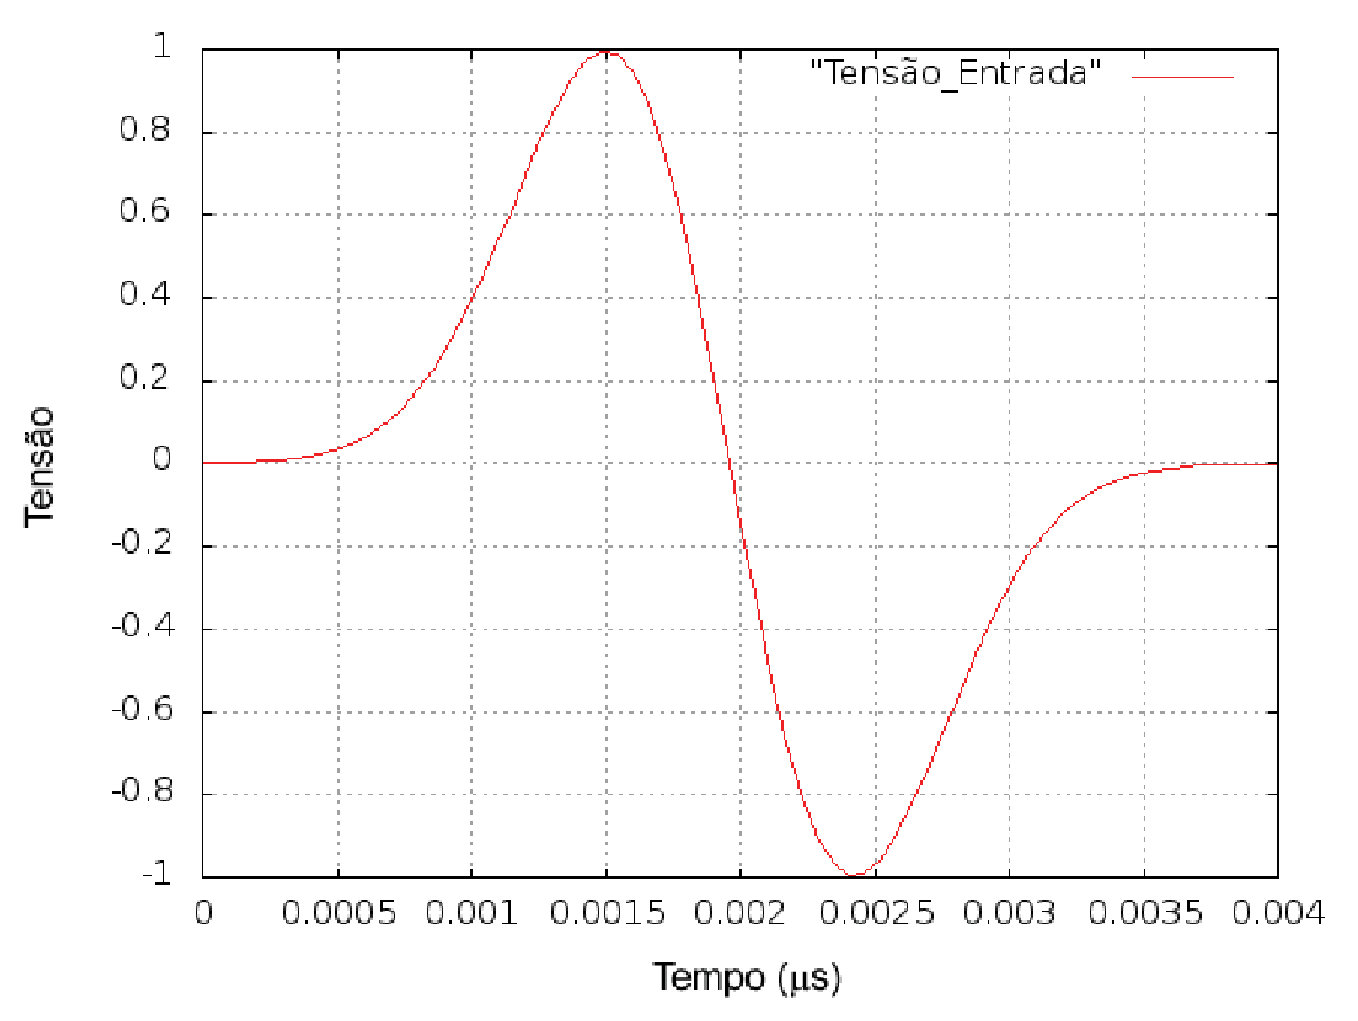
\includegraphics[scale=0.25]{t_in}}
	\end{center}
	\caption{Tensões obtidas pela simulação.}
	\label{fg:tensoes}
\end{figure}

	Por meio desses dados de entrada e saída, desejava-se calcular o perfil de potência e retardo do canal, dado por \ref{eq:potencia},para este ambiente virtual. Todavia, para que isso fosse possível, era necessário ter a resposta impulsiva $h(t)$ desse canal. A Figura~\ref{fg:dia} mostra o processo de obtenção da resposta em frequência e a Figura~\ref{fg:hf} mostra esta resposta.

\begin{equation}\label{eq:potencia}
	P_h(\tau) = |h(\tau)|^{2}
\end{equation}
\begin{figure}[!ht]
	\centering
	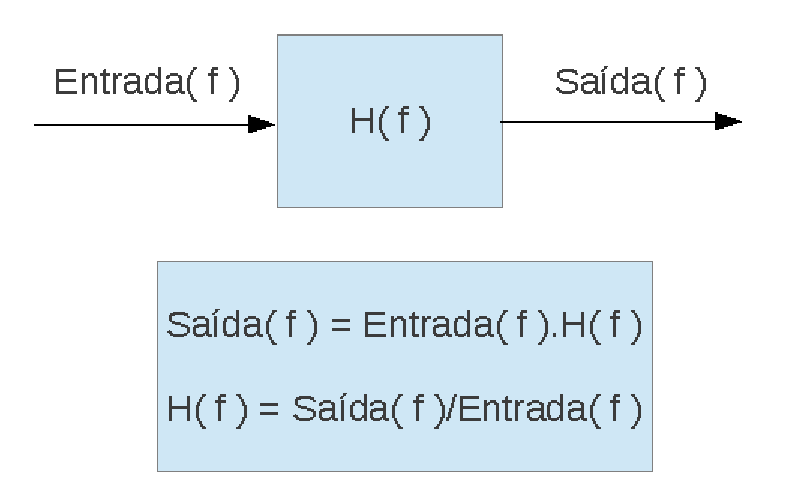
\includegraphics[scale = 0.5]{dia}
	\caption{Diagrama de bloco ilustrando a operação linear de obtenção da função de transferência $H(f)$.}
	\label{fg:dia}
\end{figure}
\begin{figure}[!ht]
	\centering
	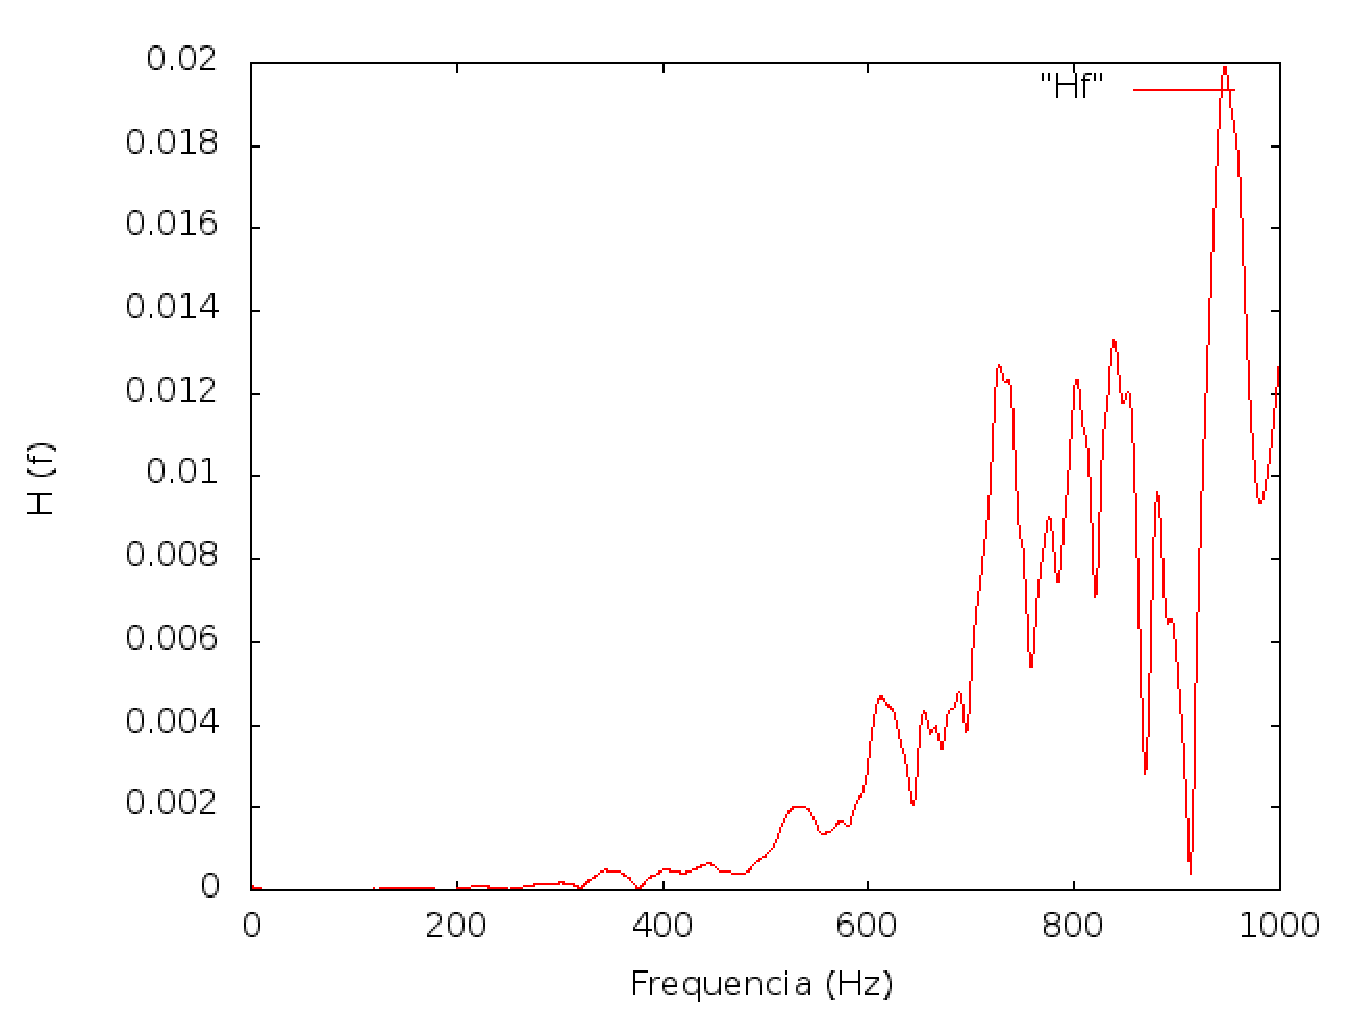
\includegraphics[scale = 0.5]{hf}
	\caption{Função de transferência $H(f)$ do canal de propagação, considerando-se os pontos T1 e R.}
	\label{fg:hf}
\end{figure}

	Logo, as tensões de entrada(referente ao ponto T1) e saída (referente ao ponto R), usando a transformada de Fourier, foram passadas para o domínio da frequência e então divididas ponto a ponto. Com isso, obteve-se a resposta em frequência, $H( f )$ da Fig.~\ref{fg:hf}. Usando a Equação~\ref{eq:ant_f}, referente a anti-transformada de Fourier, obtém-se a resposta impulsiva do canal. Através dela, foi possível comparar o perfil de potência e retardo obtido pela simulação com o medido em ~\cite{fabricio}. A Figura~\ref{fg:ms} mostra esta comparação.

\begin{equation}\label{eq:ant_f}
	h(\tau) = \mathcal{F}^{-1}{H(f)}
\end{equation}

\begin{figure}[!ht]
	\centering
	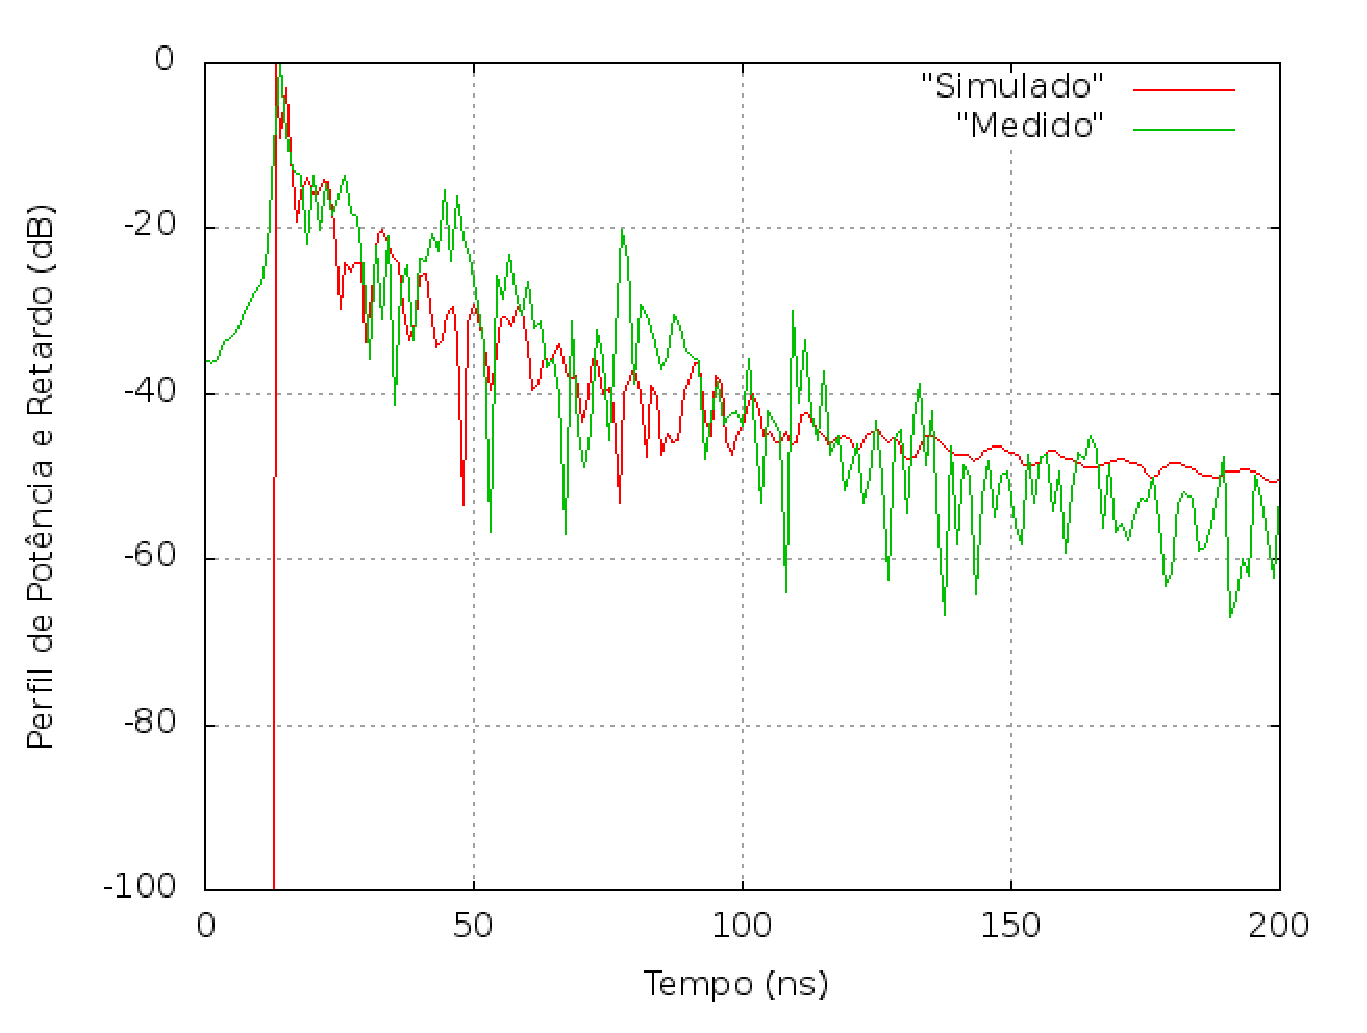
\includegraphics[scale = 0.5]{ms}
	\caption{Comparação entre medição~\cite{fabricio} e simulação referente aos pontos T1 e R.}
	\label{fg:ms}
\end{figure}
	
	\subsubsection{Caso 02}
	O mesmo processo que foi realizado no caso 1 foi refeito neste caso, diferenciando somente no posicionamento da antena transmissora(agora posicionada em T2 ). O perfil de potencia e retardo obtido foi o mostrado na Figura~\ref{fg:ms2}.

\begin{figure}[!ht]
	\centering
	\includegraphics[scale = 0.5]{ms2}
	\caption{Comparação entre medição~\cite{fabricio} e simulação referente aos ponto T2 e R.}
	\label{fg:ms2}
\end{figure}

	\subsubsection{Conclusão}
	A exelente concordância entre os resultados experimentais e simulados ocorre devido ao fato de método FDTD produzir soluções de onda completa, levando em conta todos os efeitos de refração, reflexão e difração eletromagnética em todos os pontos do domínio do problema e em todos os instantes de tempo. Desta forma, estes resultados validam a implementação da interface produzida neste trabalho. As diferenças principais ocorrem para valores abaixo de -20dB, de forma que pode-se atribuí-las a presença de ruídos e eventuais objetos pŕesentes no ambiente na hora da medição, que não foram inseridos no modelo. Ressalta-se que , mesmo abaixo de -20dB, os níveis de $h(t)$ são compatíveis com os níveis obtidos experimentalmente.
